
\documentclass[a4paper,12pt]{article}
\title{projectreport}
\usepackage[top=1in, bottom=1in, left=1in, right=1in]{geometry}
\usepackage{epsfig}
\usepackage{float}
\usepackage{multicol}
\usepackage{graphicx}
\usepackage{titlesec}
\usepackage{lipsum}
\usepackage{caption}
\usepackage{subcaption}
\usepackage{booktabs}
%\usepackage[dvips]{graphics}
\usepackage{sectsty}
\usepackage{chngcntr}
\usepackage[hidelinks]{hyperref}
\usepackage{algorithmic}
\usepackage{algorithm2e}
%\usepackage[dvips]{graphics}
\sectionfont{\centering}
%\usepackage{helvet}
%\renewcommand{\familydefault}{\sfdefault}
%\usepackage{titlesec}
%\setkomafont{section}{\normalfont\huge\sffamily\bfseries\color{blue}}
%\renewcommand{\rmdefault}{phv} % Arial
%\renewcommand{\sfdefault}{phv} % Arial
\renewcommand{\abstractname}{\large Abstract}
\counterwithin{figure}{section}
\newcommand*{\myfont}{\fontfamily{Arial}\selectfont}
\renewcommand{\baselinestretch}{1.5}


\begin{document}

\pagenumbering{gobble}
\thispagestyle{empty}
\begin{center}
\textbf{Major Project Proposal Report} \\
\textbf{On}\\
\vspace{2 mm}
\Large{\textsc{ A COMPARATIVE RESEARCH STUDY ON VIDEO SEMANTIC RECOGNITION }}   % Your Minor Project Title

\vspace{7 mm}
\large{\textbf{                  % Group members name
Submitted by 
}}
\\
\large{\textbf{                  % Group members name
12IT79 Siddharth P. Ramakrishna \\
12IT09 Anuj Kumar \\
12IT62 Rohit Kumar \\
}}

\vspace{4 mm}
Under the Guidance of,\\
\textbf{Dinesh Naik}\\         % Name of your guide
Department of Information Technology, NITK Surathkal\\
\vspace{4 mm}
\textit{Date of Submission: 3/9/2015}
\vspace{14 mm}
	
		
\includegraphics[width=1.5in,height=1.5in]
		{nitk.jpg}
 
\textbf{Department of Information Technology}

\textbf{National Institute of Technology Karnataka, Surathkal}

\textbf{2015}
\end{center}

%%%%%%%%%%%%%%%%%%%%%%%%%%% Page 3 %%%%%%%%%%%%%%%%%%%%%%%%%%%%%%%%%%%%%%


\newpage
         \begin{abstract}
The accuracy and efficiency of the Video Semantic Recognition can be improved by performing feature selection on the features that has been extracted from the video. A subset of features has been selected. The feature set is highly dimensional because a video is generally very rich in semantic. Feature selection is done for a better, compact and accurate representation of the video. Since it is difficult and time consuming to compute all the labelled videos and do a classification, the number of labelled videos is small. Nowadays, most of the applications have a large amount of unlabelled videos. And supervised feature selection will fail to realise the important features since the labelled videos are less and therefore it is difficult to do a classification to target classes. So this gives an intuition to use a mixture of labelled and unlabelled videos and apply semi supervised algorithms to select relevant features from the video such that they are discriminative to respective target classes by using effectively the information associated with the large amount of unlabeled videos. In this project, we will provide a comparative study of which algorithm has the most efficiency and accuracy under the given assumptions. Following are the three semi supervised algorithms that we will be approaching for the study – Spline Regression, Graph Based Semi Supervised Algorithm and Adaboost. In the experiments to come, a comparative study will be provided on the three typical tasks of video semantic recognition, namely – Video Concept Detection, Video Classification and Human Action Recognition. \\
\textbf{Keywords:  }\emph{Regression,Video Classification, Adaboost }
	\end{abstract}

%%%%%%%%%%%%%%%%%%%%%%%%%%% Page 4 %%%%%%%%%%%%%%%%%%%%%%%%%%%%%%%%%%%%%%

\newpage
\tableofcontents

%%%%%%%%%%%%%%%%%%%%%%%%%%% Page 5 %%%%%%%%%%%%%%%%%%%%%%%%%%%%%%%%%%%%%%

\newpage
\listoffigures

%%%%%%%%%%%%%%%%%%%%%%%%%%% Page 6 %%%%%%%%%%%%%%%%%%%%%%%%%%%%%%%%%%%%%%

\newpage	
        
\pagenumbering{arabic}

%%%%%%%%%%%%%%%%%%%%%%%%%%% Page 7 %%%%%%%%%%%%%%%%%%%%%%%%%%%%%%%%%%%%%%

\section{\fontsize{16pt}{1em} \usefont{T1}{phv}{b}{}Introduction}

Most of the applications of video semantic recognition has data represented by high dimensional feature vectors. It has been observed that one can extract high dimensional visual features which are heterogeneous from a given video frame. Features such as global like direction of edges, gabor, and color moment and some local features such as space time interest points. In this high dimensional space of observed features, it is difficult to classify video samples of different classes and is called as “curse of dimensionality” problem. And since it is known that more the number of irrelevant features, the degree of polynomial tends to increase and thus the process of training used for classification tends to be overfitting. So, this issue has to be resolved.\\
One solution to this issue is dimensionality reduction. The original high dimensional feature space is reduced onto a new reduced dimensionlaity feature space and the video samples are being represented in that new space. The two basic methods of mapping in dimensionality reduction or the other way round is done either by constructing new features or by keeping a subset of the features that has been obtained from the original space. For the former mapping, two major strands are PCA( The Principal Component Analysis ) and the Isometric Mapping of data manifolds. PCA uses the linear subspace learning and the latter uses the nonlinear manifold learning methods. In this project, the dimensionality reduction approach has been explored, making a subset of the features from the original space, and its possible applications to the video semantic recognition. \\
The common approach of dimensionality reduction, feature selection, has an important role in improving the accuracy and efficieny of analysis of the video samples. Firstly, the computations has been redduced as the new dimension of the feature subset is very low. And then the noisy ones are being removed for a efficient representation of the video samples, thus making a better classification result. \\
Algorithms to perform feature selection can be basically classified into the following groups, supervised feature selection and the unsupervised feature selection. In supervised features selection, the algorithm computes the relevance of the feature by evaluating the correlation of that feature with the target classes. Pastly, Fischer score, robust regression and regression algorithms like sparse multi output regression has been used to select the features based on the labels on the training data. Since the discriminative information is there enclosed with the labels, the supervised feature selection algorithm is able to select the discriminative features from the training data. The unsupervised feature selection algorithm uses the separability and the variance among the data to evaluate feature relevance where there are no labels in the training data. \\ The usual practice criteria that has been observed is to select some of the features that preserve the distribution of the data and structure of the data set from the entire feature set efficiently. But the difficulty here is that the label information sometimes is not directly available and therefore the unsupervised feature selection algorithm has more problems in selecting the disriminative features using the distribution and the structure of the data. \\
It has been observed that the amount of unlabeled videos are huge and getting large amount of high quality labelled videos is very difficult. Since the amount of labelled videos is fairly small, supervised feature selection algorithm will fail to find out the features that are relevant enough to discrimate them to respective target classes. Therefore a need for semi supervised feature selection algorithm approach could be used to identify the most relevant features that are discriminative enough to target classes. In order to make use of the labelled and the unlabelled video samples, the semi superised feature selection algorithm makes use of the distribution and the structure of the data to evaluate the relevance of the features. Several semi supervised feature selection algorithms based on the spectral assumption, the geometry of distribution of data, and others. \\
So, in this project, we propose a comparative study for semi supervised feature selection via the following semi supervised algorithms like the Spline regression, the graph based semi supervised algorithm and the adaboost algorithm. \\
In the experiments to come, standard benchmark video samples as training data sets are used to provide a comparative study on the performance of video semantic recognition by semi supervised feature selection algorithms which basically corresponds to the three important video semantic recognition taks. A comparative study on the performance of video semantic recognition using the semi supervised feature selection algorithms will be provided.

\vspace{0.5cm}
\
\newpage
\section{\fontsize{16pt}{1em} \usefont{T1}{phv}{b}{} Literature Survey}


\subsection{\usefont{T1}{phv}{b}{it} Background}
Semi Supervised classification is a special form of classification. Traditional classifiers use only labeled data (feature / label pairs) to train. Labeled instances however are often difficult, expensive, or time consuming to obtain, as they require the efforts of experienced human annotators. Meanwhile unlabeled data may be relatively easy to collect, but there has been few ways to use them. Semi-supervised learning addresses this problem by using large amount of unlabeled data, together with the labeled data, to build better classifiers. Because semi-supervised learning requires less human effort and gives higher accuracy, it is of great interest both in theory and in practice. Labels are hard to obtain while unlabeled data are abundant, therefore semi-supervised learning is a good idea to reduce human labor and improve accuracy. Anecdotally, the fact that unlabeled data do not always help semi-supervised learning has been observed by multiple researchers. For example people have long realized that training Hidden Markov Model with unlabeled data (the Baum-Welsh algorithm, which by the way qualifies as semi-supervised learning on sequences) can reduce accuracy under certain initial conditions (Elworthy, 1994). \\
Many semi supervised learning methods are there. Some often-used methods include: EM with generative mixture models, self-training, co-training, transductive support vector machines, and graph-based methods. \\
There is no direct answer to the question hich method suits the best. Because labeled data is scarce, semi- supervised learning methods make strong model assumptions. Ideally one should use a method whose assumptions fit the problem structure. This may be difficult in reality. Nonetheless we can try the following checklist: Do the classes produce well clustered data? If yes, EM with generative mixture models may be a good choice; Do the features naturally split into two sets? If yes, co-training may be appropriate; Is it true that two points with similar features tend to be in the same class? If yes, graph-based methods can be used; Already using SVM? Transductive SVM is a natural extension; Is the existing supervised classifier complicated and hard to modify? Self-training is a practical wrapper method. \\
Semi-supervised learning methods use unlabeled data to either modify or reprioritize hypotheses obtained from labeled data alone. \\

‘Transductive learning’ will be used to contrast inductive learning. A learner is transductive if it only works on the labeled and unlabeled training data, and cannot handle unseen data. The early graph-based methods are often transductive. Inductive learners can naturally handle unseen data. People sometimes use the analogy that transductive learning is take-home exam, while inductive learning is in-class exam.
\\
.In order to improve the accuracy and efficiency for the video semantic recognition, one can perform feature selection on the video features extracted to choose a subset of the features from the set of high dimensional features to have a better, compact and accurate video presentation. Yang, Yan, Ma, Sebe, N and Zhou( 2014 ) developed an iterative algorithm for the experiment and were able to prove its convergency. In the experiments, the three important and typical tasks of semantic recognition in videos, i.e, video classification, human action recognition and video concept detection, are used to demonstrate that the proposed algorithm semi supervised feature selection via spline regression achieves good performance when compared with the other state-of-the-art methods.
\\
 The automatic understanding of the audio and the visual content for the multi media retrieval is not an easy task, because the meaning basically the appearance of a certain event or a concept is strongly determined by the contextual information present. Ewerth and Bernd( 2007 ) show that it is quite possible to adaptively grasp and learn the appearance of some certain objects or some events for a particular video( test video ) using unlabeled data so that it can improve over subsequent retrieval process. So, basically first an initial model is obtained using supervised learning making use of a set of appropriate training videos. Then, this model is being used to rank the shots for each test video Vi separately. This ranking system is used to label the most important and the least important shots in the video Vi for further use as training or the input data in a semi supervised learning process. So basically using these labeled training data, important features are being selected for the concept in consideration for the video Vi. Then, the two additional classifiers are being trained on the data of this video which are automatically labeled. Adaboost and SVM( Support Vector Machines ) are being incorporated for the feature selection process and the classification ensemble process. And then finally the newly obtained trained classifiers and initial model act as an ensemble. They performed experiments on the TRECVID 2005 video data and demonstrated the feasibility of proposed learning scheme for the certain high level concepts. \\
The multimedia applications require video management and it is becoming more and more desirable and important to give proper video data index techniques which are capable of representing the semantics in video data that are rich in nature. In most real-time applications, there is a need for efficiently query processing which is one of the other for the use of such techniques. Serhan, Khatib, Ghafoor, Kashyap( 2000 ) have presented the models that can use the object motion information to characterize the further events that can allow further subsequent retrieval. Different algorithms for different search in terms of spatiotemporal cases in temporal and spatials translation and scaling invariance have been in development using various image processing and signal processing techniques. PICTURESQUE ( pictorial information and content transformation unified retrieval engine for spatiotemporal queries ) to basically prove the methods that has been proposed. With the development of such technologies, it will enable true multimedia search engines which will allow searching of the video data in digital form and indexing based on the true content.\\
The problem for the graph classification has attracted great interest in recent times. Currently going research assumes that there is large number of labeled training graphs available. But most of the times labels of the graph data are really very expensive and are difficult to obtain, and at the same there are large amounts of unlabeled graph data present. Kong and Yu( 2010 ) developed the algorithm whose aim is to efficiently search for the optimal sub graph features containing both the labeled and the un labeled graphs.
\\
 The accuracy and efficiency of the Video Semantic Recognition can be improved by performing feature selection on the features that has been extracted from the video. A subset of features has been selected. The feature set is highly dimensional because a video is generally very rich in semantic. Han, Yang, Ma, Yan, Sebe, Zhou( 2014 ) show that Feature selection is done for a better, compact and accurate representation of the video. Since it is difficult and time consuming to compute all the labelled videos and do a classification, the number of labelled videos is small.
 \\
\subsection{\usefont{T1}{phv}{b}{it} Outcome of Literature Survey}


\subsection{\usefont{T1}{phv}{b}{it}Problem Statement}
Given a large set of labeled and unlabeled training videos, apply semi supervised learning techniques in order to semantically categorize them. Based on the type of data received and assumptions made on the training data, provide a comprehensive study of which algorithms work best under what circumstances.


\subsection{\usefont{T1}{phv}{b}{it}Objectives}
\begin{enumerate}
\item Process the key frames and generate the feature set
\item Apply the semi supervised algorithms on the featured data set to generate reduced feature set
\item Obtain results and plot graphs to determine which algorithms work well with the given data set
\item Varying some of the assumptions and heuristics involved, check to see whether that has an impact on the performance of a given algorithm 

\end{enumerate}


\newpage
\section{\fontsize{16pt}{1em} \usefont{T1}{phv}{b}{}Research Methodology}
\begin{enumerate}
\item
\textbf{Spline Regression}

A spline curve is a mathematical representation which allow a user to design and control the shape of complex curves and surfaces. The user enters a sequence of points, and a curve is constructed whose shape closely follows this sequence.The points are called control points. A curve that actually passes through each control point is called an interpolating curve and a curve that passes near to the
control points but not necessarily through them is called an approximating curve.


Cubic Splines are used for the following reasons
\begin{enumerate}
\item it is the lowest degree polynomial that can support an inflection
\item it is very well behaved numerically – that means that the curves will
usually be smooth and not jumpy

\end{enumerate}

To make more complex curves we used the concepts of piecewise curve fitting and parameterization. The conditions for piece wise curve fitting are as follows:

\begin{enumerate}
\item We require that each curve segment pass through its control points. Thus,
\begin{equation}
f(xi) = yi,
\end{equation}
 and,
 \begin{equation}
 fi(xi+1) = yi+1.
 \end{equation}
  This enforces C0 continuity – that is,where the curves join they meet each other.
\item We require that the curve segments have the same slope where they join
together. Thus, 
\begin{equation}
f'(i)(xi+1) = f'(i+1)(xi+1).
\end{equation} This enforces C1 continuity –that is that slopes match where the curves join.
\item The curve segments have the same curvature where they join together. Thus, 
\begin{equation}
f''(i)(xi+1) = f''(i+1)(xi+1).
\end{equation}

This enforces C2 continuity – that curvatures match at the join.


\end{enumerate}

Semi Supervised Feature Selection using Spline Regression – Methodology
\begin{figure}

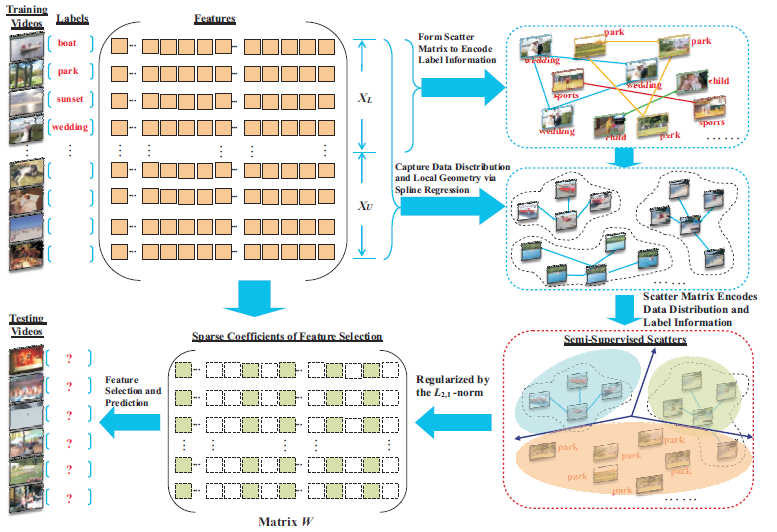
\includegraphics[width=1.0\textwidth]{./spline.jpg}
\caption{ Supervised Feature Selection Via Spline Regression }
\end{figure}

Given a large data set of labelled and unlabelled videos, where the size of unlabelled is greater than the size of labelled, we employ semi supervised feature selection using spline regression in the following manner :
\begin{enumerate}
\item We create a feature matrix with the entire data set.
\item We create a scatter matrix with only the labelled set to encode label information
\item With the unlabelled set,we apply spline regression to capture data distribution and local geometry
\item We create a scatter matrix with the same and we end up with semi supervised scatters in the process
\item After regularization via the L21 norm, the new matrix W will be sparse in rows which makes it ideal for feature selection
\item The top features are taken into consideration and is used to classify the test videos

\end{enumerate}

\begin{figure}

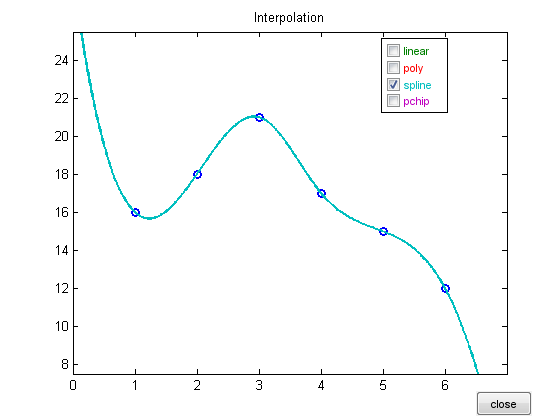
\includegraphics[width=1.0\textwidth]{./spline2.jpg}
\caption{ Supervised Feature Selection Via Spline Regression Interpolation }
\end{figure}


Some of the challenges that spline regression faces is that there is a tendency to overfit and how these control points are determined. Fortunately, many programming language implementations of this automatically assign these control points in such a way that piecewise smooth curves are generated which follow the aformentioned three conditions. The resultant curve generated out of this process is made to best fit the data without overfitting the data.
\item 
\textbf{Graph Based Semi Supervised Algorithm} \\
In this algorithm, the idea is to efficiently search for the optimal sub graph features containing both the labeled and the un labeled graphs. This algorithm is different from the existing feature selection processes in vector spaces which has the assumption that the feature set is given, but this algorithm has the semi supervised feature selection being performed on graph data in a proceeding way together with the sub graph feature mining process. Also we develop a feature evaluation criteria in order to estimate the usefulness of subgraph features based upon both the labeled graphs and the unlabeled graphs. Then we need to develop an algorithm to efficiently search for optimal subgraph features by judiciously pruning/cutting the sub graph feature space. \\

\begin{figure}

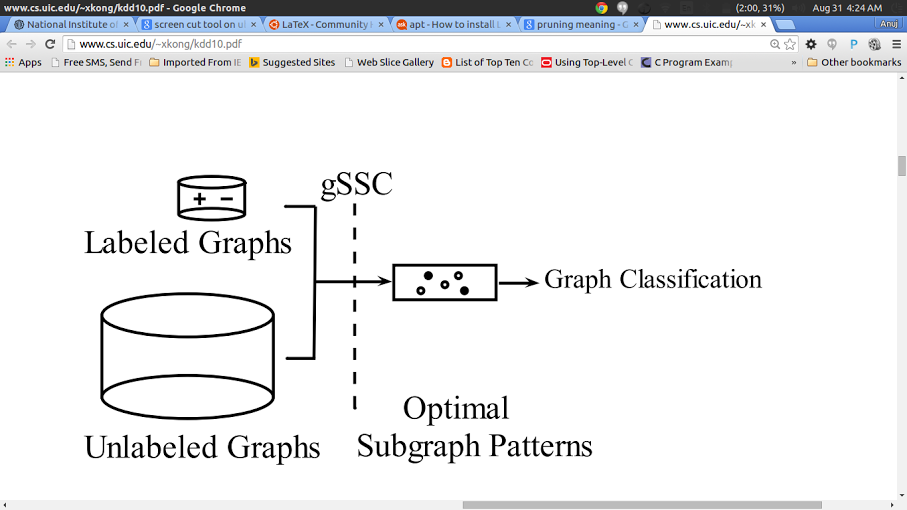
\includegraphics[width=1.0\textwidth]{./graph1.jpg}
\caption{ Graph Semi Supervised Mechanism }
\end{figure}


One of the major difficulty associated with the graph classification is in the structure of graph which gets complex at times and there will be lack of vector representations. So, selecting a proper set of features for data in graph is an important for graph classification process. As it is known that generating large amount of labeled data is really expensive and difficult to obtain. At the same time there is tremendous large amount of un labeled data available. Thus it is very much desirable that the large amounts of un labeled graphs can be used to have a better feature selection for graphs, and imporve the graph classification performances.\\
\begin{figure}
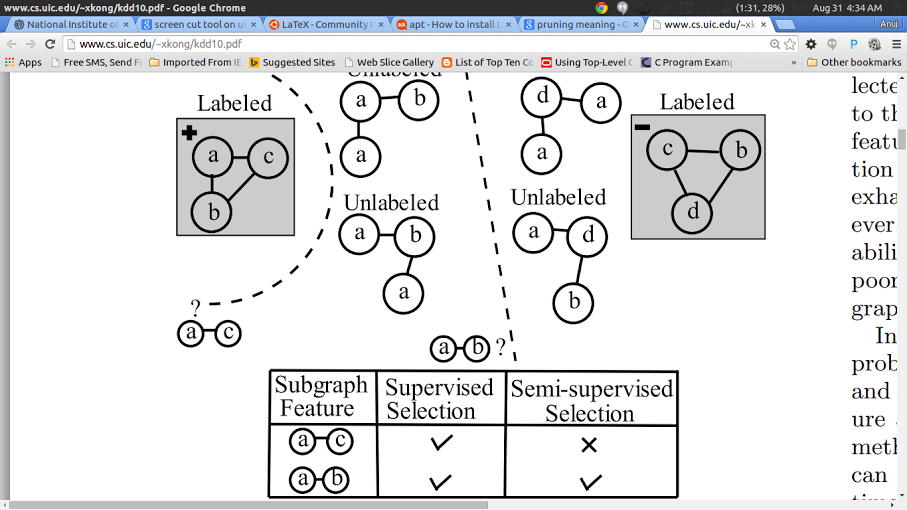
\includegraphics[width=1.0\textwidth]{./graph2.jpg}
\caption{ Graph Semi Supervised Algorithm Example }
\end{figure}

Consider this example for the graph based semi supervised feature selection algorithm \\
Let us consider a dataset with four un labeled graphs and two labeled graphs. Now in the two labeled graphs one can observe that the two discriminative features are “a-b” and “a-c”. It is very clear that the subgraph feature “a-b” is more useful than “a-c” in order to separate the unlabeled graphs. This happens because the un labeled graphs are not at all separable on the basis of “a-c”. \\
\end{enumerate}
\newpage
\section{\fontsize{16pt}{1em} \usefont{T1}{phv}{b}{}Results and Analysis}
The time complexity of the clustering algorithm is O(n) where n is number of iterations for which the algorithm runs. The complexity of the DoM calculation algorithm is O(n*n*k) where n is number of services in the test data that are considered and O(k) is the number of inputs and outputs for each service.

We have calculated DoM for 50 services in the given OWL-S TC collection. The figure 5.1 shows the DoM matrix for the first 20 services
\\
\begin{figure}[htb]
\centering
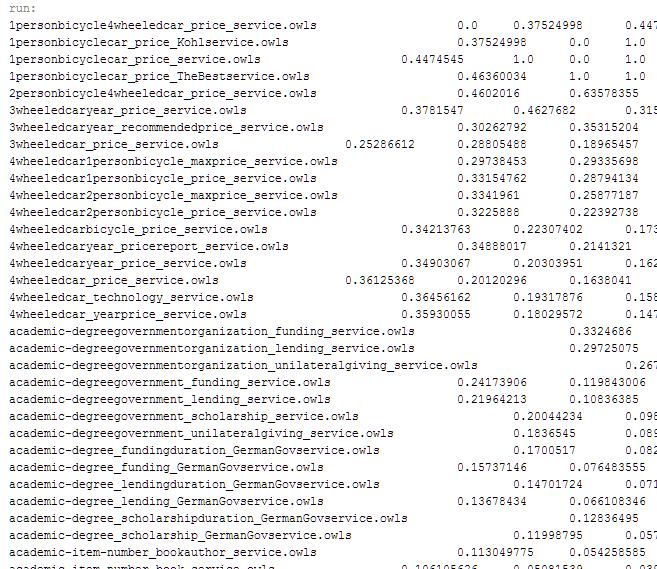
\includegraphics[scale=1]{./values.jpg}
\caption{Matrix of  between services}
\label{fig:label} 
\end{figure}
The figures 5.2 and 5.3 show the initial and final distribution of the services in the grid
\newpage
\begin{figure}[htb]
\centering

\caption{Service distribution before Clustering}
\label{fig:label} 
\end{figure}
\newpage
\begin{figure}[htb]
\centering
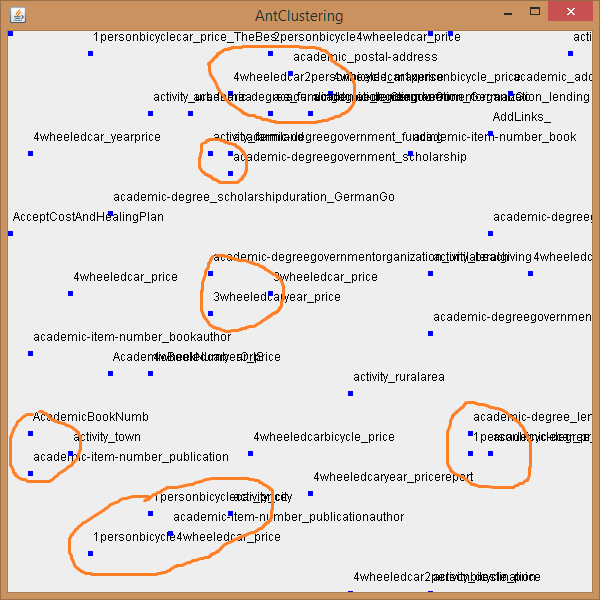
\includegraphics[scale=1]{./final.jpg}
\caption{Service distribution before Clustering}
\label{fig:label} 
\end{figure}

The ant based clustering is highly dependent on neighborhood size , threshold , number of ants and the memory of an ant .



\newpage
\section{\fontsize{16pt}{1em} \usefont{T1}{phv}{b}{}Conclusion \& Future Work}

The ant based approach can be improved further by using the concepts of parallel computing. Each ant agent can be given its own thread and every ant can continue to move without being affected by status of other ant agent. This would greatly decrease the computation time of the algorithm. Also other bio-inspired techniques like Bird flocking techniques could be used. 


%create bibtex files for references
\newpage
\bibliographystyle{plain}
\begin{thebibliography}{9}
\bibitem{p1}
An ant-inspired approach for semantic web service clustering
Chifu, \\V.R. ; Pop, C.B. ; Salomie, I. ; Dinsoreanu, M. ; Acretoaie, V. ; David, T. 
\\Roedunet International Conference (RoEduNet), 2010 9th 
\\Publication Year: 2010 , Page(s): 145	- 150 
\bibitem{p1}
 D. Skoutas, D. Sacharidis, V. Kantere and T. Sellis. "Efficient Semantic Web Service Discovery in Centralized and P2P Environments". LNCS vol. 5318/2010, pp. 583-598, 2010. 
\bibitem{api1}
WSDL parser Java API : \url{http://easywsdl.ow2.org/}
\bibitem{api2}
OWL / RDF parser Java API:\url{https://jena.apache.org/}
\end{thebibliography}
\end{document}